\documentclass[10pt,a4paper]{article}
\usepackage[margin=0.7in]{geometry}
\usepackage[T1]{fontenc}
\usepackage{lmodern}
\usepackage{amsmath,amssymb,booktabs,graphicx,microtype}
\usepackage[font=small,labelfont=bf,skip=4pt,hypcap=false]{caption}
\usepackage[hidelinks]{hyperref}
\usepackage{enumitem}
\setlength{\parindent}{0pt}
\setlength{\parskip}{5pt}
\setlength{\abovedisplayskip}{6pt}
\setlength{\belowdisplayskip}{6pt}
\setlist{nosep,leftmargin=*}
\newcommand{\ones}{\mathbf{1}}
\newcommand{\Sig}{\widehat{\Sigma}}
\title{\vspace{-1.8em}\textbf{Mean--Variance Portfolio Selection}\\[-2pt]
\large FIN6131 Portfolio and Asset Management: Assignment 1}
\author{}
\date{19 September 2026}
\hypersetup{pdftitle={FIN6131 Assignment 1: Mean-Variance Portfolio Selection},pdfsubject={Nine-ETF efficient frontiers and out-of-sample robustness}}
\begin{document}
\maketitle
\vspace{-2.4em}

\section{Data, estimation, and portfolio theory}
\textbf{Research question.} Does the in-sample benefit of allowing short sales survive a chronological holdout? Following the mean--variance framework of Markowitz~\cite{source1}, this study separates the attainable risk--return trade-off from the reliability of estimated optimal weights. The principal finding is that short selling improves the fitted frontier, but extreme leverage makes unrestricted tangency fragile out of sample.

\textbf{Sample and provenance.} Nine USD-denominated ETFs span US large-cap equities (SPY), Nasdaq-100 (QQQ), US small-cap equities (IWM), developed ex-US equities (EFA), emerging equities (EEM), long US Treasuries (TLT), investment-grade corporate bonds (LQD), gold (GLD), and US REITs (VNQ). The five-year return window is 19 September 2021 through 18 September 2026. Yahoo adjusted closes account for splits and distributions~\cite{source3}; they serve as a historical total-return proxy. Direct \texttt{yfinance} access was blocked, so the same provider's public chart responses were obtained through a browser on 19 September 2026. The executable notebook includes the documented \texttt{yfinance} download option~\cite{source2} and a verified offline snapshot. Raw responses, exact URLs, and checksums are archived.

There are 1,256 aligned price observations per ETF, including the prior close of 17 September 2021, yielding \textbf{1,255 daily returns} from 20 September 2021 onward. There are no missing cells, duplicate dates, imputed prices, or dropped trading rows. For adjusted price $P_{it}$, estimation uses
\[
 r_{it}=\log(P_{it}/P_{i,t-1}),\qquad
 \widehat\mu=252\bar r,\qquad
 \Sig=\frac{252}{T-1}\sum_{t=1}^{T}(r_t-\bar r)(r_t-\bar r)^\top.
\]
The sample covariance is positive definite (condition number 238.69). Full-sample annual log means range from $-8.66\%$ for TLT to $17.99\%$ for GLD. These are historical estimates, not forecasts. Asset statistics and the complete covariance matrix appear in the notebook.

\textbf{Optimization and the efficient set.} With $\ones^\top w=1$, expected return and variance are $w^\top\widehat\mu$ and $w^\top\Sig w$. For each target $m$, solve
\[
 \min_w\;\tfrac12w^\top\Sig w
 \quad\text{subject to}\quad \ones^\top w=1,\quad w^\top\widehat\mu=m,
 \quad \begin{cases}w\in\mathbb R^9 &(\mathrm{U}:\text{ shorts allowed}),\\
 w_i\ge0 &(\mathrm{L}:\text{ long-only}).\end{cases}
\]
The global minimum variance portfolio (MVP) removes the target constraint; the efficient frontier is the upper branch starting at that regime's MVP. The budget condition remains in the ``unconstrained'' case. With $A=\ones^\top\Sig^{-1}\ones$, $B=\ones^\top\Sig^{-1}\widehat\mu$, $C=\widehat\mu^\top\Sig^{-1}\widehat\mu$, and $D=AC-B^2$, unrestricted solutions satisfy
\[
 w_G=\frac{\Sig^{-1}\ones}{A},\qquad
 w(m)=\Sig^{-1}\!\left(\frac{C-Bm}{D}\ones+\frac{Am-B}{D}\widehat\mu\right),\qquad
 \sigma^2(m)=\frac{Am^2-2Bm+C}{D}.
\]
Long-only portfolios are solved by checked SLSQP quadratic programs. Feasible-set inclusion implies that short-sale restrictions cannot lower minimum variance at a common target return. They also bound attainable means between the smallest and largest asset means; unrestricted target returns have no finite upper bound.

\textbf{Tangency and cash allocation.} At the stipulated annual $r_f=3\%$, tangency maximizes $S(w)=(w^\top\widehat\mu-r_f)/\sqrt{w^\top\Sig w}$. For $e=\widehat\mu-r_f\ones$, $w_T=\Sig^{-1}e/(\ones^\top\Sig^{-1}e)$ in regime U; its normalization is positive in both estimation windows. For L, the convex program $\min_{z\ge0}z^\top\Sig z$ subject to $e^\top z=1$, followed by $w=z/(\ones^\top z)$, avoids a local ratio optimum. Allocation $y$ to tangency and $1-y$ to cash gives the CAL $\mu_C=r_f+S_T\sigma_C$ for $y\ge0$. Lending corresponds to $0\le y\le1$; $y>1$ assumes borrowing at the same rate. The risky-sleeve short-sale restriction does not itself forbid borrowing cash.

\textbf{Return-convention caveat.} As requested, these optimization formulas use annualized \emph{asset log-return} moments and subtract 0.03 directly. Weighted asset log returns are not exact portfolio log returns: the frontier, Sharpe objective, and CAL are conventional MPT approximations, particularly under leverage. The holdout below instead compounds exact weighted simple returns. Converting 3\% to $\log(1.03)$ changes full-sample long-only tangency weights by at most 0.060 percentage points, but does not remove the broader approximation.

\newpage
\section{Full-sample frontier and economic interpretation}
\begin{center}
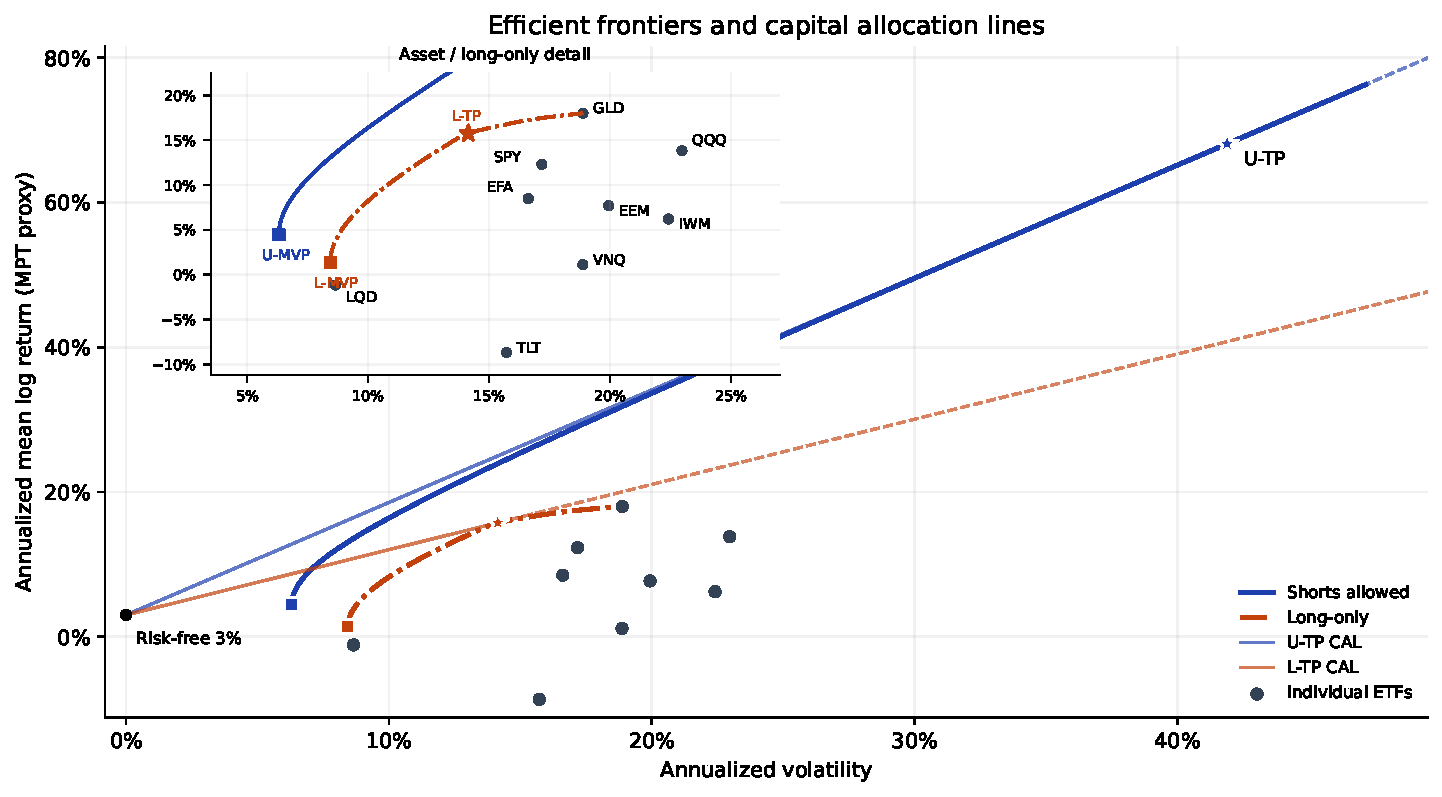
\includegraphics[width=0.96\linewidth]{outputs/figures/frontiers.pdf}
\captionof{figure}{Both efficient frontiers, four optimized portfolios, individual ETFs, and both CALs. The inset labels assets and low-risk portfolios on the same axis definitions. Solid CAL segments involve lending; dashed extensions assume borrowing. The unrestricted frontier is shown over a finite range, not truncated economically.}
\label{fig:frontiers}
\end{center}
\vspace{-5pt}
\begin{minipage}[t]{0.47\linewidth}
\centering
\captionof{table}{Full-sample weights (\%).}
\label{tab:weights}
\small\setlength{\tabcolsep}{4pt}
\begin{tabular}{lrrrr}
\toprule
ETF & U-MVP & L-MVP & U-TP & L-TP \\
\midrule
SPY & 54.21 & 6.47 & 519.43 & 39.42 \\
QQQ & -35.24 & 0.00 & -159.19 & 0.00 \\
IWM & -10.47 & 0.00 & -104.04 & 0.00 \\
EFA & -13.57 & 0.00 & -36.34 & 0.00 \\
EEM & 7.90 & 0.00 & -50.89 & 0.00 \\
TLT & -56.48 & 0.00 & -135.38 & 0.00 \\
LQD & 157.56 & 85.06 & -7.02 & 0.00 \\
GLD & 4.87 & 8.48 & 160.36 & 60.58 \\
VNQ & -8.78 & 0.00 & -86.92 & 0.00 \\
\bottomrule
\end{tabular}

\end{minipage}\hfill
\begin{minipage}[t]{0.51\linewidth}
\centering
\captionof{table}{Annual fitted MPT statistics.}
\label{tab:full}
\small\setlength{\tabcolsep}{4pt}
\begin{tabular}{lrrrr}
\toprule
Portfolio & $\mu$ (\%) & $\sigma$ (\%) & Sharpe & Gross ($	imes$) \\
\midrule
U-MVP & 4.48 & 6.31 & 0.234 & 3.491 \\
L-MVP & 1.35 & 8.44 & -0.196 & 1.000 \\
U-TP & 68.10 & 41.89 & 1.554 & 12.596 \\
L-TP & 15.75 & 14.14 & 0.901 & 1.000 \\
\bottomrule
\end{tabular}

\par\vspace{7pt}\raggedright
\footnotesize U = shorts allowed; L = long-only; TP = tangency portfolio. Gross exposure is $\sum_i|w_i|$ relative to net wealth. Displayed weights are rounded; unrounded weights sum to one. Zero weights are active nonnegativity constraints.
\end{minipage}

\textbf{Diversification versus leverage.} U-MVP achieves 6.31\% volatility, compared with 8.44\% for L-MVP and 8.66\% for the least-volatile individual ETF, LQD. Covariance hedges therefore reduce risk below that of any single asset. The unrestricted solution uses a 157.56\% LQD holding and a $-56.48\%$ TLT position, among other offsets; its 3.49-times gross exposure is not a low-leverage investment. The long-only MVP places 85.06\% in LQD, sacrificing hedge flexibility. Its 1.35\% fitted mean lies below cash's 3\%: it minimizes \emph{risky-asset variance}, not investor utility, and is dominated by cash once the risk-free asset is admitted.

\textbf{The price of the fitted Sharpe improvement.} U-TP raises fitted Sharpe from L-TP's 0.901 to 1.554, but requires 12.60-times gross exposure: 519.43\% SPY and 160.36\% GLD, financed by shorts in the other seven ETFs. Its 68.10\% fitted mean accompanies 41.89\% volatility, not an arbitrage. L-TP instead allocates 39.42\% to SPY and 60.58\% to GLD, with 15.75\% fitted mean and 14.14\% volatility. Holding many available ETFs is not necessarily optimal when their covariances overlap; nevertheless, a two-asset solution is exposed to concentration and sample-specific mean estimates. Restricting shorts lowers the fitted Sharpe by construction, while potentially reducing estimation-error amplification.

\newpage
\section{Chronological robustness and limitations}
The first three calendar years contain \textbf{754 training returns} (through 18 September 2024); the last two contain \textbf{501 holdout returns} (19 September 2024--18 September 2026). All four optimizers are refitted using training data only. Those \emph{target} weights remain frozen and are restored by daily rebalancing; equal weighting uses the identical convention with $w_i=1/9$. This is not fixed-share buy-and-hold. Training L-TP holds 26.58\% SPY and 73.42\% GLD, whereas training U-TP has 14.68-times gross exposure. Full-sample weights never enter the holdout evaluation.

For each holdout date, $R_{pt}=\sum_iw_i[\exp(r_{it})-1]$ and $W_t=\prod_{s\le t}(1+R_{ps})$. The first holdout return uses the final training close. Realized Sharpe is $\sqrt{252}(\bar R_p-R_{f,d})/s(R_p)$, with $R_{f,d}=1.03^{1/252}-1$; CAGR is $W_N^{252/N}-1$. Drawdown uses $W_0=1$ in the running peak. Costs, taxes, margin calls, and stock-loan fees are omitted.
\begin{center}
\captionof{table}{Holdout results from frozen training weights; drawdowns are signed peak-to-trough losses.}
\label{tab:oos}
\small\begin{tabular}{lrrrrr}
\toprule
Portfolio & CAGR (\%) & Vol. (\%) & Sharpe & Max DD (\%) & Total (\%) \\
\midrule
U-MVP & 7.53 & 5.52 & 0.808 & -5.93 & 15.53 \\
L-MVP & 9.19 & 8.27 & 0.747 & -6.72 & 19.10 \\
U-TP & 61.18 & 56.83 & 1.075 & -64.99 & 158.32 \\
L-TP & 28.15 & 18.98 & 1.247 & -18.38 & 63.75 \\
Equal & 14.75 & 12.55 & 0.924 & -11.48 & 31.47 \\
\bottomrule
\end{tabular}

\end{center}
\vspace{-9pt}
\begin{center}
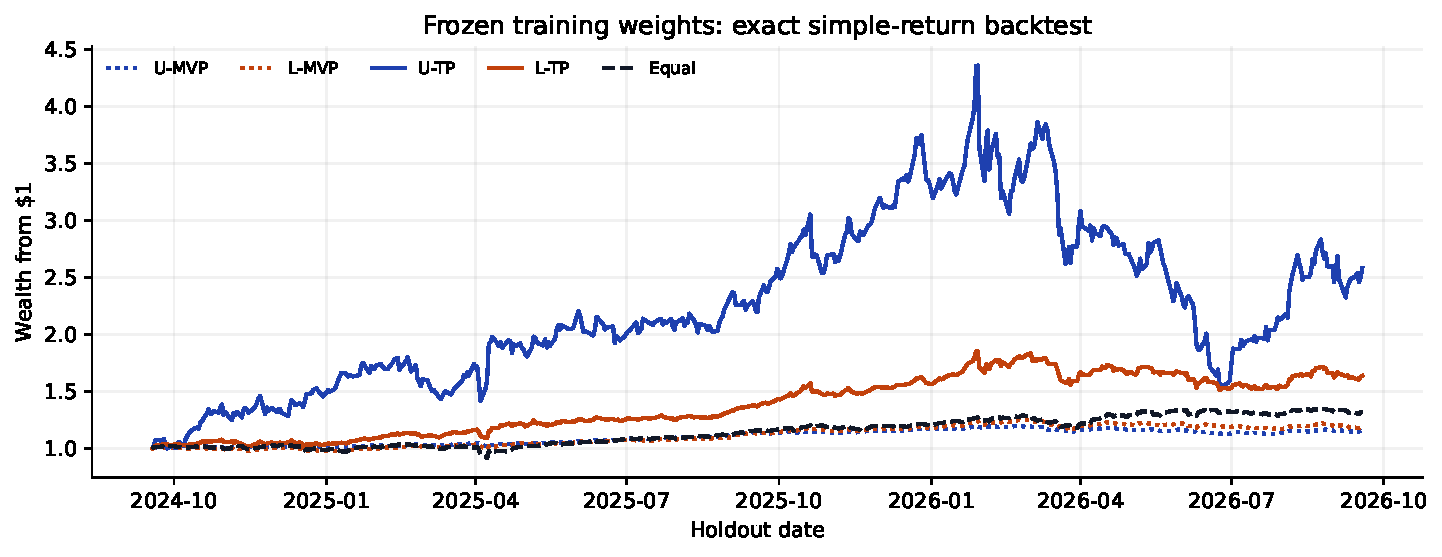
\includegraphics[width=0.90\linewidth,height=1.85in,keepaspectratio]{outputs/figures/oos_wealth.pdf}
\captionof{figure}{Exact compounded holdout wealth, with all strategies starting from one dollar.}
\end{center}
\vspace{-7pt}

\textbf{Interpretation.} L-TP delivers the highest holdout Sharpe, 1.247, versus 1.075 for U-TP and 0.924 for equal weighting. Its 28.15\% CAGR exceeds the benchmark's 14.75\%, but volatility (18.98\% versus 12.55\%) and drawdown (18.38\% versus 11.48\% in magnitude) are also larger: it does not dominate equal weighting on every criterion. U-TP delivers the largest total gain, 158.32\%, yet loses 64.99\% from its running peak. Both MVPs reduce volatility and drawdown relative to equal weighting but have lower CAGR and Sharpe. Thus the optimizer's objective matters: minimum variance is not maximum realized reward per unit risk.

\textbf{What the robustness check does and does not establish.} U-TP's training Sharpe proxy of 1.817 falls to a realized holdout Sharpe of 1.075, alongside volatility rising from 43.89\% to 56.83\%; the comparison also changes from log-moment to simple-return measurement. Long-only tangency wins on holdout Sharpe in this sample, consistent with constraints limiting unstable offsetting bets, but this one split cannot establish causality or statistical superiority. Historical means are noisy; covariances vary across regimes; overlapping equity exposures amplify estimation sensitivity. Surviving ETF selection, revised adjusted-price histories, fat tails, and omitted shorting/turnover costs further limit implementability. Future work should test rolling holdouts, mean/covariance shrinkage, leverage caps, and realistic financing and rebalancing costs rather than tune on this holdout.

\textbf{Reproducibility.} The standalone notebook embeds the checked CSV and all numerical functions; seed 6131 and locked dependencies support reruns. All 98 tests pass, including isolated offline notebook execution. Independent SLSQP and analytic weights agree within $3.23\times10^{-7}$; common-target frontier dominance and a holdout-perturbation no-lookahead check pass. Tables and plots are generated from the same executed results. These are historical research results, not investment recommendations.

\begingroup
\footnotesize
\setlength{\parskip}{0pt}
\begin{thebibliography}{3}
\setlength{\itemsep}{0pt}
\bibitem{source1} H. Markowitz (1952). Portfolio Selection. \emph{The Journal of Finance}, 7(1), 77--91. \href{https://onlinelibrary.wiley.com/doi/10.1111/j.1540-6261.1952.tb01525.x}{doi:10.1111/j.1540-6261.1952.tb01525.x}.
\bibitem{source2} yfinance. \emph{download API documentation}. \url{https://ranaroussi.github.io/yfinance/reference/api/yfinance.download.html} (accessed 19 September 2026).
\bibitem{source3} Yahoo Finance. \emph{What is the adjusted close?} \url{https://help.yahoo.com/kb/SLN28256.html} (accessed 19 September 2026). Raw data provenance: repository \texttt{assignment1/data/metadata.json}.
\end{thebibliography}
\endgroup
\end{document}
